\chapter{含风电的电力系统调度模型及附加结果}
\label{cha:cons-flexibility-CHP-Thermal}

\section{CHP建模及灵活性约束}
为聚焦于分析灵活风机在降低系统弃风水平、增强系统灵活性方面的优势,本节假定区域内供热需求均由CHP满足,系统无电热泵、储热等装置。CHP的供热与供电特性相互耦合,可由热电联合运行可行域描述。CHP的热电可行域主要有凸可行域与非凸可行域两种,如图~\ref{fig:Append-CHP-Convexity}所示。

\begin{figure}[H] % use float package if you want it here
  \centering
  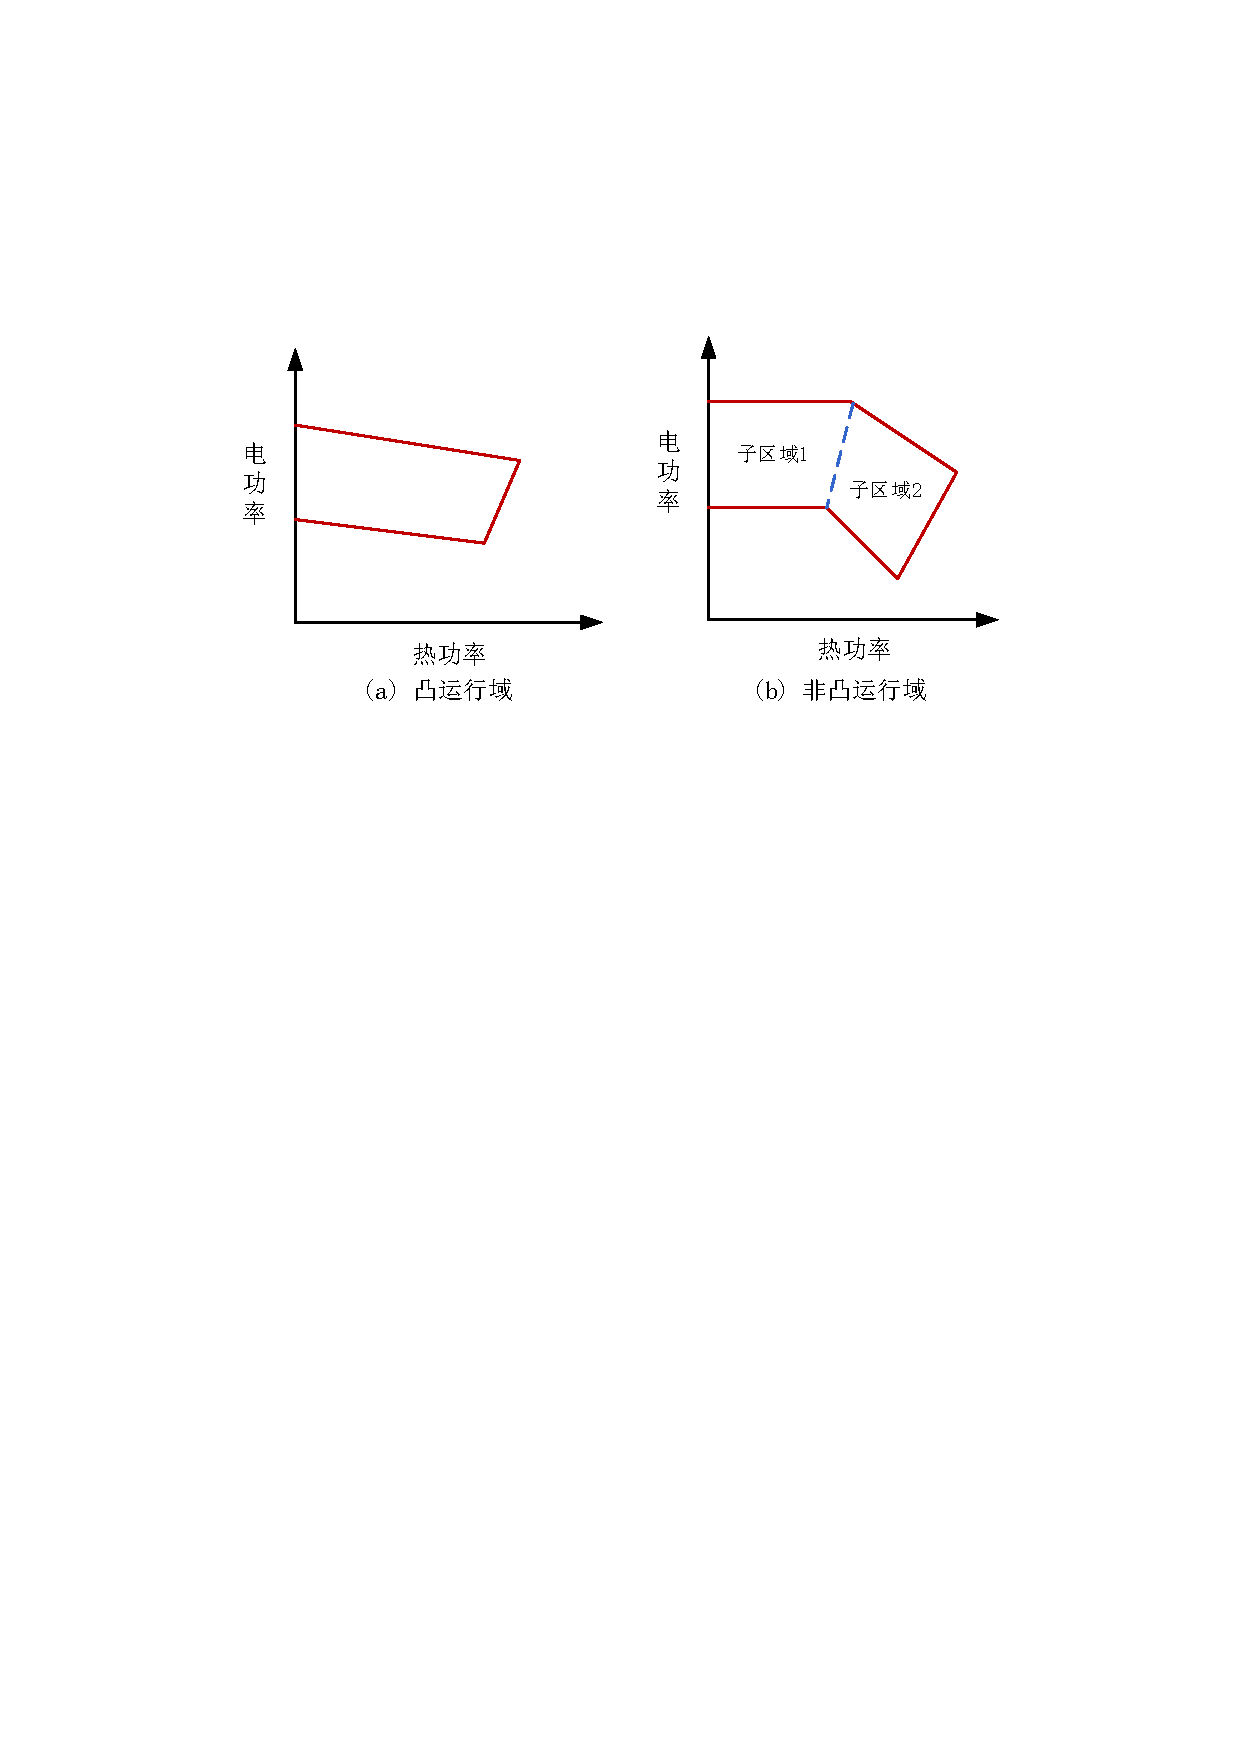
\includegraphics[scale=0.75]{figures/Chap-Append-CHP-Convexity.pdf}
  \caption{CHP的典型凸与非凸热电可行域}
  \label{fig:Append-CHP-Convexity}
\end{figure}

对于满足凸性的CHP热电可行域,其供热与供电功率及成本可表示为极点的凸组合~\cite{CHP-Model-03, CHP-Model-CXY-15,IES-Model-CXY-18},即
\begin{equation}
\label{eq:convex-CHP-PQ}
p_{i,t}^c = \sum\limits_{k = 1}^M {\alpha _{i,t}^kx_i^k,q_{i,t}^c = \sum\limits_{k = 1}^M {\alpha _{i,t}^ky_i^k} ,C_{i,t}^c = \sum\limits_{k = 1}^M {\alpha _{i,t}^kc_i^k} }, \forall i,t
\end{equation}
其中,$(x_i^k,y_i^k,c_i^k)$ 为极点$k$对应的电功率、热功率及运行成本,$\alpha _{i,t}^k$ 为各极点线性组合系数,满足$\sum\limits_{k{\rm{ = }}1}^M {\alpha _{i,t}^k}  = I_{i,t}^{c(1)}$。对于不满足凸性的CHP热电可行域,可将区域划分为几个凸区域,进而针对每个区域采用类型凸性的方法(\ref{eq:convex-CHP-PQ})进行建模。如图\ref{fig:Append-CHP-Convexity}(b)所示,假定非凸热电可行域可分为两个凸区域,则CHP的供热与供电功率满足,
\begin{equation}
\label{eq:non-convex-CHP-PQ}
p_{i,t}^c = \sum\limits_{k = 1}^{{M_1}} {\alpha _{i,t}^kx_{i1}^k} {\rm{ + }}\sum\limits_{k = 1}^{{M_2}} {\beta _{i,t}^kx_{i2}^k} ,q_{i,t}^c = \sum\limits_{k = 1}^{{M_1}} {\alpha _{i,t}^ky_{i,1}^k} {\rm{ + }}\sum\limits_{k = 1}^{{M_2}} {\beta _{i,t}^ky_{i2}^k}, \forall i,t
\end{equation}
其中,$(\alpha _{i,t}^k,\beta _{i,t}^k)$ 为各个凸子区域的系数,并满足,
\begin{equation}
\sum\limits_{k = 1}^{{M_1}} {\alpha _{i,t}^k}  = I_{_{i,t}}^{c(1)},\sum\limits_{k = 1}^{{M_2}} {\beta _{i,t}^k}  = I_{i,t}^{c(2)},\;\forall i,t
\end{equation}
其中,$(I_{_{1,t}}^{c(1)},I_{_{2,t}}^{c(2)})$ 为表征机组运行状态的0-1量; $I_{i,t}^{c(1)} = 1$ 表示CHP运行于凸区域1,$I_{i,t}^{c(2)} = 1$ 表示CHP机组运行于凸区域2。

令$I_{i,t}^c$为表征CHP机组运行状态的布尔量,其满足
\begin{equation}
0 \le I_{i,t}^c = I_{i,t}^{c(1)} + I_{i,t}^{c(2)} \le 1, \; \forall i, t
\end{equation}

CHP的燃料成本由供热功率以及电功率共同决定,其值可由热电可行域中各极点成本的凸组合表示,即
\begin{equation}
C_{i,t}^c = \sum\limits_{k = 1}^{{M_i}} {\alpha _{_{i,t}}^kc_{i,1}^k}  + \sum\limits_{k = 1}^{{M_i}} {\beta _{_{i,t}}^kc_{i,2}^k}, \; \forall i,t
\end{equation}

CHP机组的启动成本约束可描述为,
\begin{equation}
S_{i,t}^c \ge {\lambda _i}(I_{i,t}^c - I_{i,t - 1}^c), \; \forall i,t
\end{equation}
其中,$\lambda _i$ 为CHP机组$i$的启动成本。

%\section{CHP灵活性约束}
%\subsection{CHP爬坡约束}
CHP机组的爬坡约束可建模为\cite{UC-Model-06, CHP-Model-CXY-15, IES-Model-CXY-18},
\begin{subequations}
\begin{gather}
p_{i,t}^c - p_{i,t - 1}^c \le R_i^uI_{i,t - 1}^c + S_i^u(I_{i,t}^c - I_{i,t - 1}^c) + \bar P_i^c(1 - I_{i,t}^c), \forall i,t \\
p_{i,t}^c - p_{i,t - 1}^c \ge  - (R_i^dI_{i,t}^c + S_i^d(I_{i,t - 1}^c - I_{i,t}^c)), \forall i,t
\end{gather}
\end{subequations}
其中,$R_i^d$ 与 $R_i^u$ 分别为向上爬坡与向下爬坡限制;$S_i^d$ 与 $S_i^u$ 分别为启动或停机爬坡限制,$\bar P_i^c$  为CHP机组$i$的最大电功率输出,满足
\cite{IES-Model-CXY-18}
\begin{subequations}
\begin{gather}
\bar P_i^c = \max (x_i^k),\;\;k = 1,\cdots,M, \forall i\\
P_{i,t}^c \le \bar P_i^cI_{i,t + 1}^c + S_i^d(I_{i,t}^c - I_{i,t + 1}^c), \forall i,t
\end{gather}
\end{subequations}
%\subsection{CHP运行时间约束}

CHP机组$i$的最小运行时间约束可建模为~\cite{UC-Model-06,IES-Model-CXY-18},
\begin{subequations}
\begin{gather}
\sum\limits_{t = 1}^{{G_i}} {(1 - I_{i,t}^c) = 0}, \forall i,t  \\
\sum\limits_{v = t}^{t + T_i^{c,U} - 1} {(I_{i,v}^c)} \ge T_i^{c,U}(I_{i,t}^c - I_{i,t - 1}^c), \;\;t = {G_i}^c + 1,\cdots,T - T_i^{c,U} + 1, \forall i\\
\sum\limits_{v = t}^T {(I_{i,v}^c - (I_{i,t}^c - I_{i,t-1}^c)} ) \ge 0, \;\;\;t = T - T_i^{c,U} + 2,\cdots,T, \forall i
\end{gather}
\end{subequations}
相应地,最小停机时间约束可建模为~\cite{UC-Model-06,IES-Model-CXY-18},
\begin{subequations}
\begin{gather}
\sum\limits_{t = 1}^{{G_i}} {I_{i,t}^c = 0}, \forall i,t \\
\sum\limits_{v = t}^{t + T_i^{c,D} - 1} {(1 - I_{i,v}^c)}  \ge T_i^{c,D}(I_{i,t - 1}^c-I_{i,t}^c), \;\;t = {G_i} + 1,\cdots,T - T_i^{c,D} + 1, \forall i\\
\sum\limits_{v = t}^T {(1 - I_{i,v}^c - (I_{i,t - 1}^c - I_{i,t}^c))}  \ge 0, \;\;t = T - T_i^{c,D} + 2,\cdots,T, \forall i
\end{gather}
\end{subequations}
其中,$T_i^{c,U}$ 与 $T_i^{c,D}$ 分别表示CHP机组$i$的最小运行时间与最小停机时间; ${G_i^c}$ 为与CHP 机组$i$的初始运行状态相关的常数,若机组$i$在初始时刻处于启动状态,则${G_i^c}$ 为机组可以停机需要最小的时间间隔;若机组$i$在初始时刻处于停机状态,则${G_i}$  为机组可以启动需要的最小时间间隔。

\section{火电机组灵活性约束}
火电机组$i$的爬坡约束满足\cite{UC-Model-06, CHP-Model-CXY-15, IES-Model-CXY-18},
\begin{subequations}
\begin{gather}
p_{i,t}^e - p_{i,t - 1}^e \le R_i^uI_{i,t - 1}^c + S_i^u(I_{i,t}^e - I_{i,t - 1}^e) + {{\bar {\rm A}}_i}(1 - I_{i,t}^e), \forall i,t \\
p_{i,t}^e - p_{i,t - 1}^e \ge  - (R_i^dI_{i,t}^e + S_i^d(I_{i,t - 1}^e - I_{i,t}^e)), \forall i,t \\
p_{i,t}^e \le {{\bar {\rm A}}_i}I_{i,t + 1}^e + S_i^d(I_{i,t}^e - I_{i,t + 1}^e), \forall i,t
\end{gather}
\end{subequations}
其中,$R_i^d$ 与 $R_i^u$ 分别为机组$i$的向上与向下爬坡限制,其它变量说明可参见正文第~\ref{sec:ca-wt-power-energy-pene}节。

火电机组的最小运行时间约束可建模为\cite{UC-Model-06, CHP-Model-CXY-15},
\begin{subequations}
\begin{gather}
\sum\limits_{t = 1}^{{G_i}} {(1 - I_{i,t}^e) = 0}, \forall i,t \\
\sum\limits_{v = t}^{t + T_i^{e,U} - 1} {(I_{i,v}^e)}  \ge T_i^{e,U}(I_{i,t}^e - I_{i,t - 1}^e), \;\;t = {G_i^e} + 1,\cdots,T - T_i^{e,U} + 1, \forall i\\
\sum\limits_{v = t}^T {(I_{i,v}^e - (I_{i,t}^e - I_{i,t - 1}^e)} ) \ge 0, \;\;t = T - T_i^{e,U} + 2,\cdots,T, \forall i
\end{gather}
\end{subequations}
相应地,最小停机时间约束可建模为\cite{UC-Model-06, CHP-Model-CXY-15},
\begin{subequations}
\begin{gather}
\sum\limits_{t = 1}^{{G_i}} {I_{i,t}^e = 0}, \forall i,t \\
\sum\limits_{v = t}^{t + T_i^{e,D} - 1} {(1 - I_{i,v}^c)}\ge T_i^{e,D}(I_{i,t -1}^e-I_{i,t}^e), \;\;t = {G_i^e} + 1,\cdots,T -T_i^{e,D} + 1, \forall i \\
\sum\limits_{v = t}^T {(1 - I_{i,v}^e -(I_{i,t - 1}^e -I_{i,t}^e))} \ge 0, \;\;t = T - T_i^{e,D} + 2,\cdots,T,\forall i
\end{gather}
\end{subequations}
其中,$T_i^{e,U}$与$T_i^{e,D}$分别表示机组$i$的最小运行时间与最小停机时间;${G_i^e}$ 为允许机组启停状态变化的时间间隔。

\section{典型~CHP~机组参数}
正文第~\ref{sec:ca-wt-CF-eva}节含风电的电力系统调度算例中使用的典型CHP机组的运行可行域极点参数如表~\ref{tab:CHP-para-typical}及表~\ref{tab:CHP-para-typical-2}所示, 数据整理自文献~\inlinecite{CHP-Data-Source-18} 附录材料。

\begin{table}[htb]
  \centering
  \begin{minipage}[t]{0.8\linewidth} % 如果想在表格中使用脚注,minipage是个不错的办法
  \caption{典型~CHP~热电可行域参数}
  \label{tab:CHP-para-typical}
    \begin{tabularx}{\linewidth}{ccccc}
      \toprule[1.5pt]
      {\heiti 极点} & {\heiti CHP-1 热功率} & {\heiti CHP-1 电功率} & {\heiti CHP-2 热功率} & {\heiti CHP-2 电功率} \\\midrule[1pt]
      \#1   & 0      & 170 MW &  0     & 180 MW\\
      \#2	& 59.48 MW	 & 147 MW  & 361.39 MW & 235 MW \\
      \#3	& 106.67MW & 186  MW& 361.39 MW & 240 MW\\
      \#4	& 59.48 MW  & 200  MW& 0      & 300 MW \\
      \#5	& 0	     & 200  MW& 0      & 300 MW\\
      \#6	& 0	     & 200  MW& 0      & 300 MW\\
      \bottomrule[1.5pt]
    \end{tabularx}
  \end{minipage}
\end{table}

\begin{table}[htb]
  \centering
  \begin{minipage}[t]{0.8\linewidth} % 如果想在表格中使用脚注,minipage是个不错的办法
  \caption{典型~CHP~热电可行域参数(续)}
  \label{tab:CHP-para-typical-2}
    \begin{tabularx}{\linewidth}{ccccc}
      \toprule[1.5pt]
       {\heiti 极点} & {\heiti CHP-3 热功率} & {\heiti CHP-3 电功率} & {\heiti CHP-4 热功率} & {\heiti CHP-4 电功率} \\\midrule[1pt]
      \#1   & 0      & 154 MW  &  0     & 155 MW \\
      \#2	& 45.45 MW	 & 130 MW  & 181.94 MW & 155 MW \\
      \#3	& 100   MW & 173  MW & 181.94 MW & 193 MW\\
      \#4	& 100   MW & 190  MW & 49.17  MW & 220 MW\\
      \#5	& 45.45	MW & 210  MW & 0      & 220 MW\\
      \#6	& 0	     & 210  MW& 0      & 220 MW\\
      \bottomrule[1.5pt]
    \end{tabularx}
  \end{minipage}
\end{table}

\section{不同风电装机容量下电量平衡对比图}
\begin{figure}[H] % use float package if you want it here
  \centering
  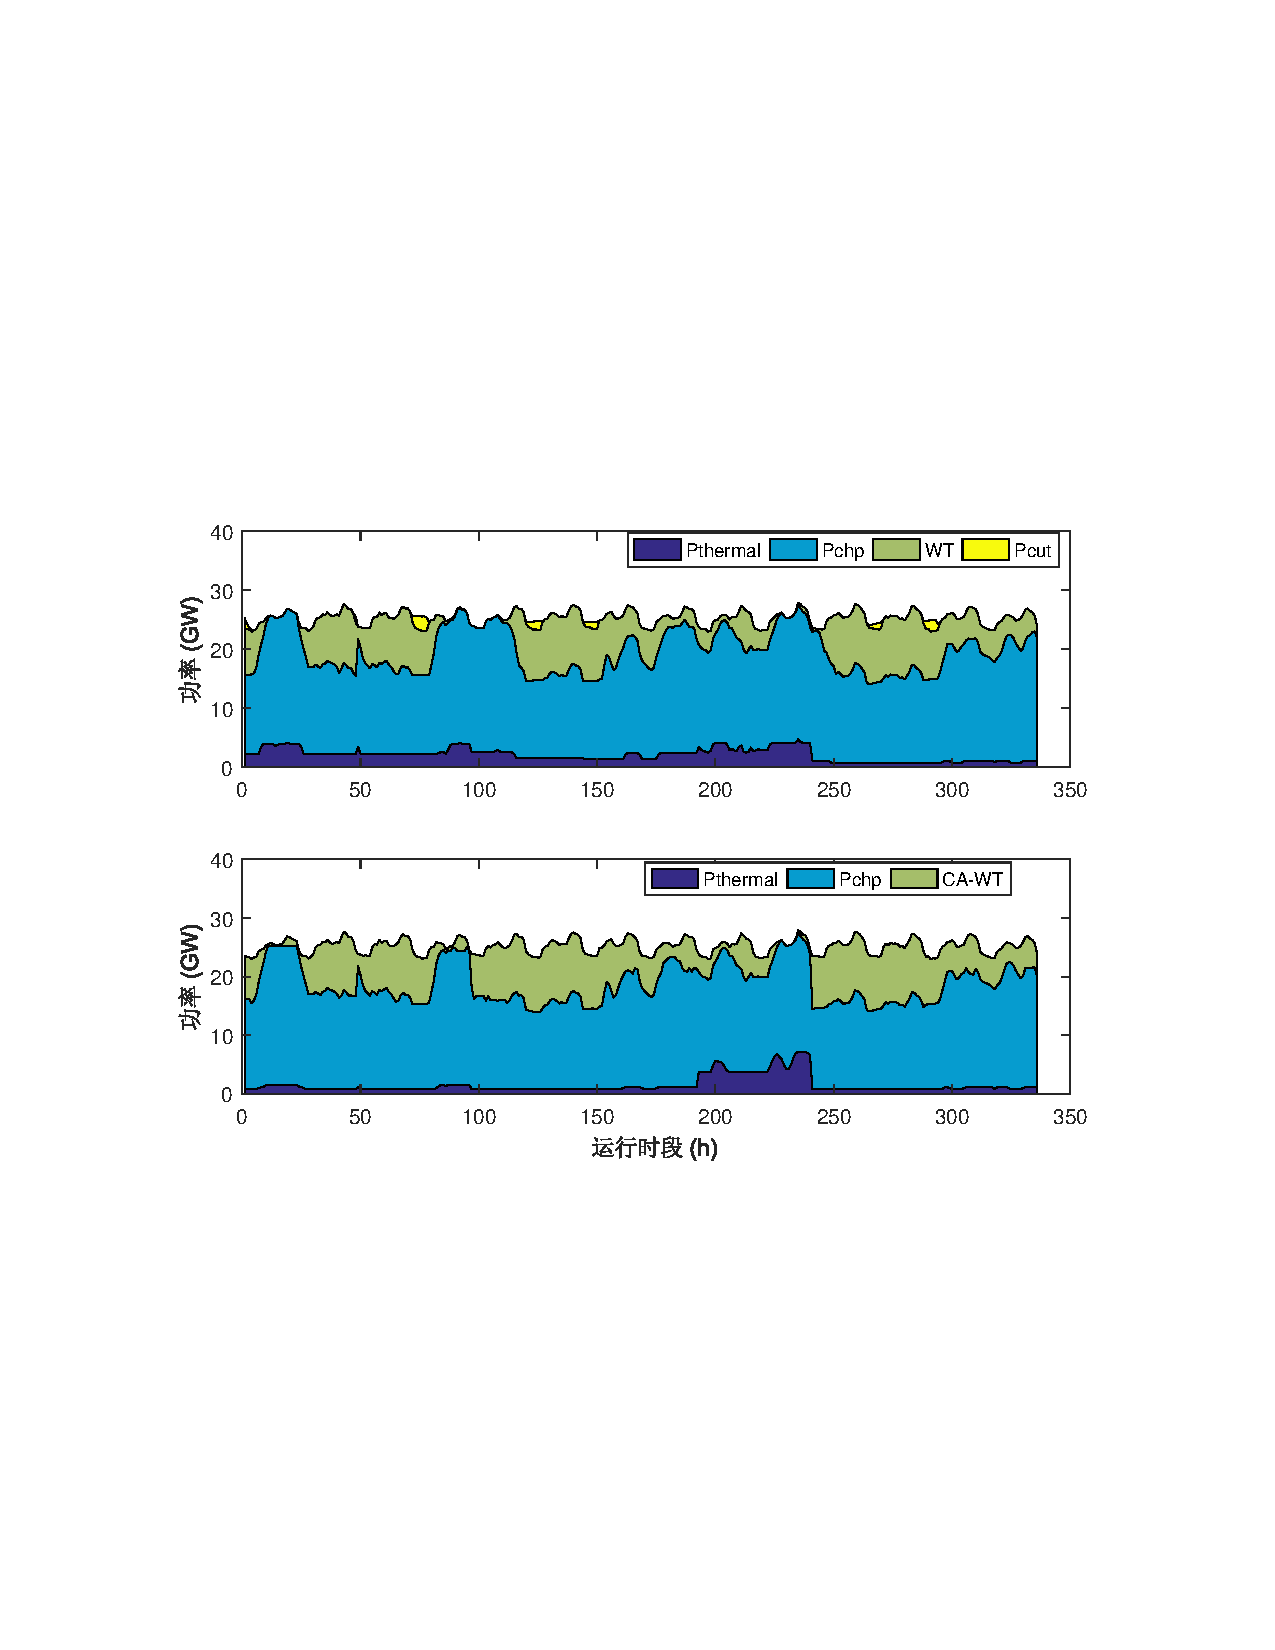
\includegraphics[scale=0.85]{figures/Chap5-Power-Balance-10G-WT.pdf}
  \caption{10GW传统风机与灵活风机电量平衡图}
  \label{fig:Power-Balance-10G-WT}
\end{figure}


\begin{figure}[H] % use float package if you want it here
  \centering
  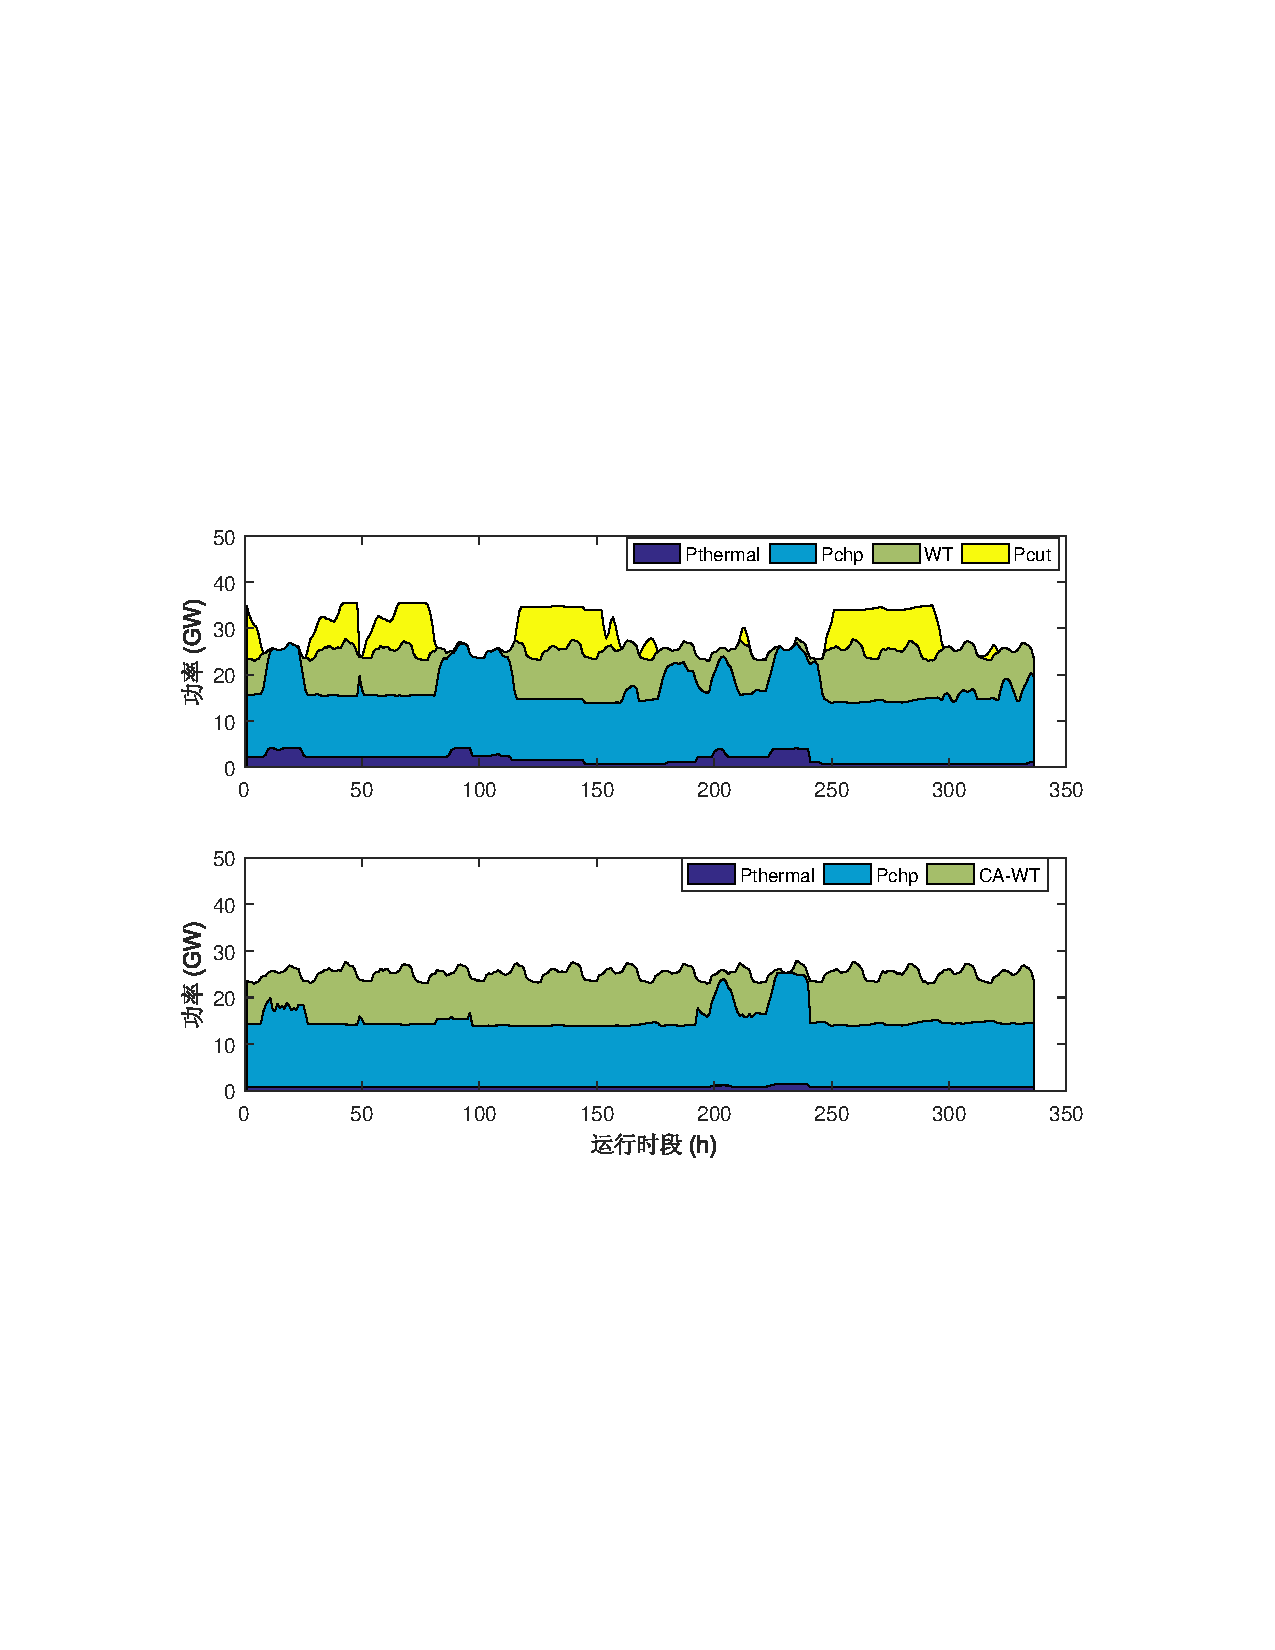
\includegraphics[scale=0.85]{figures/Chap5-Power-Balance-20G-WT.pdf}
  \caption{20GW传统风机与灵活风机电量平衡图}
  \label{fig:Power-Balance-20G-WT}
\end{figure}

\begin{figure}[H] % use float package if you want it here
  \centering
  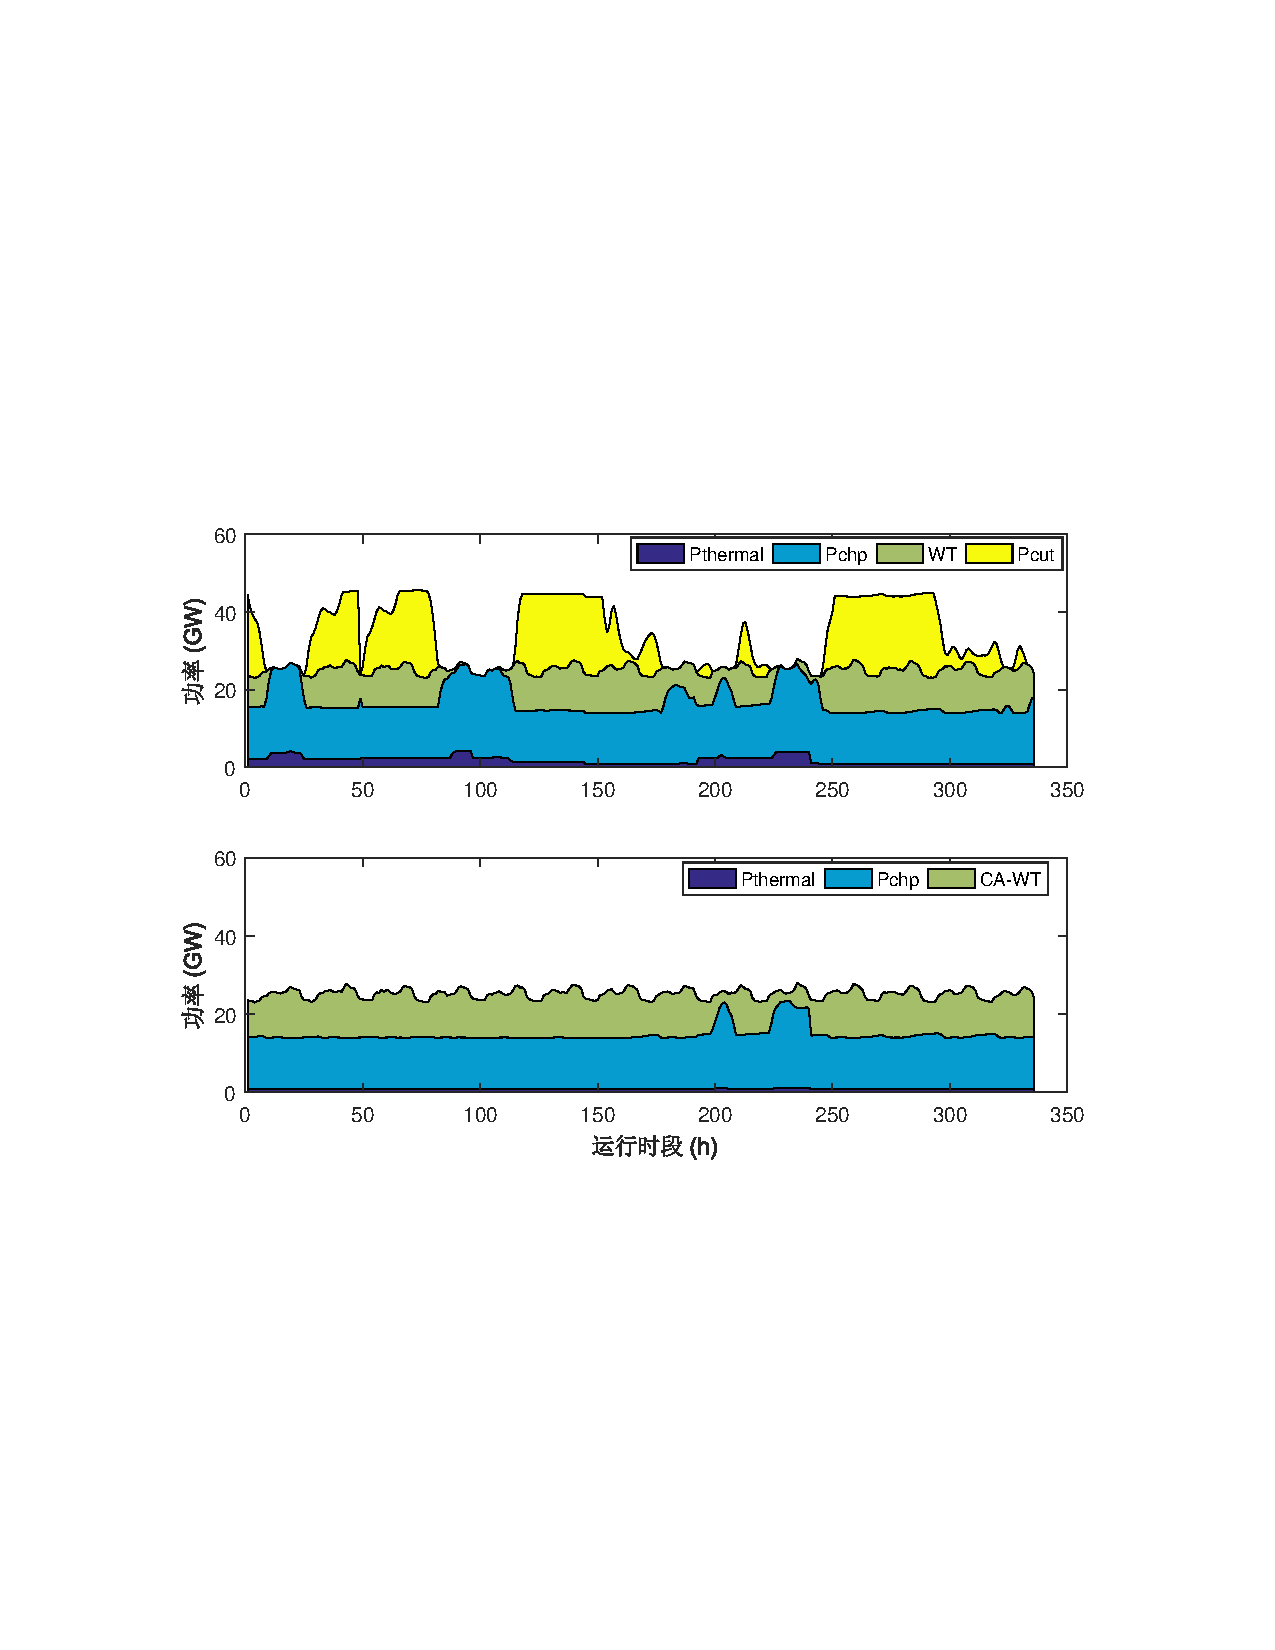
\includegraphics[scale=0.85]{figures/Chap5-Power-Balance-30G-WT.pdf}
  \caption{30GW传统风机与灵活风机电量平衡图}
  \label{fig:Power-Balance-30G-WT}
\end{figure}

\begin{figure}[H] % use float package if you want it here
  \centering
  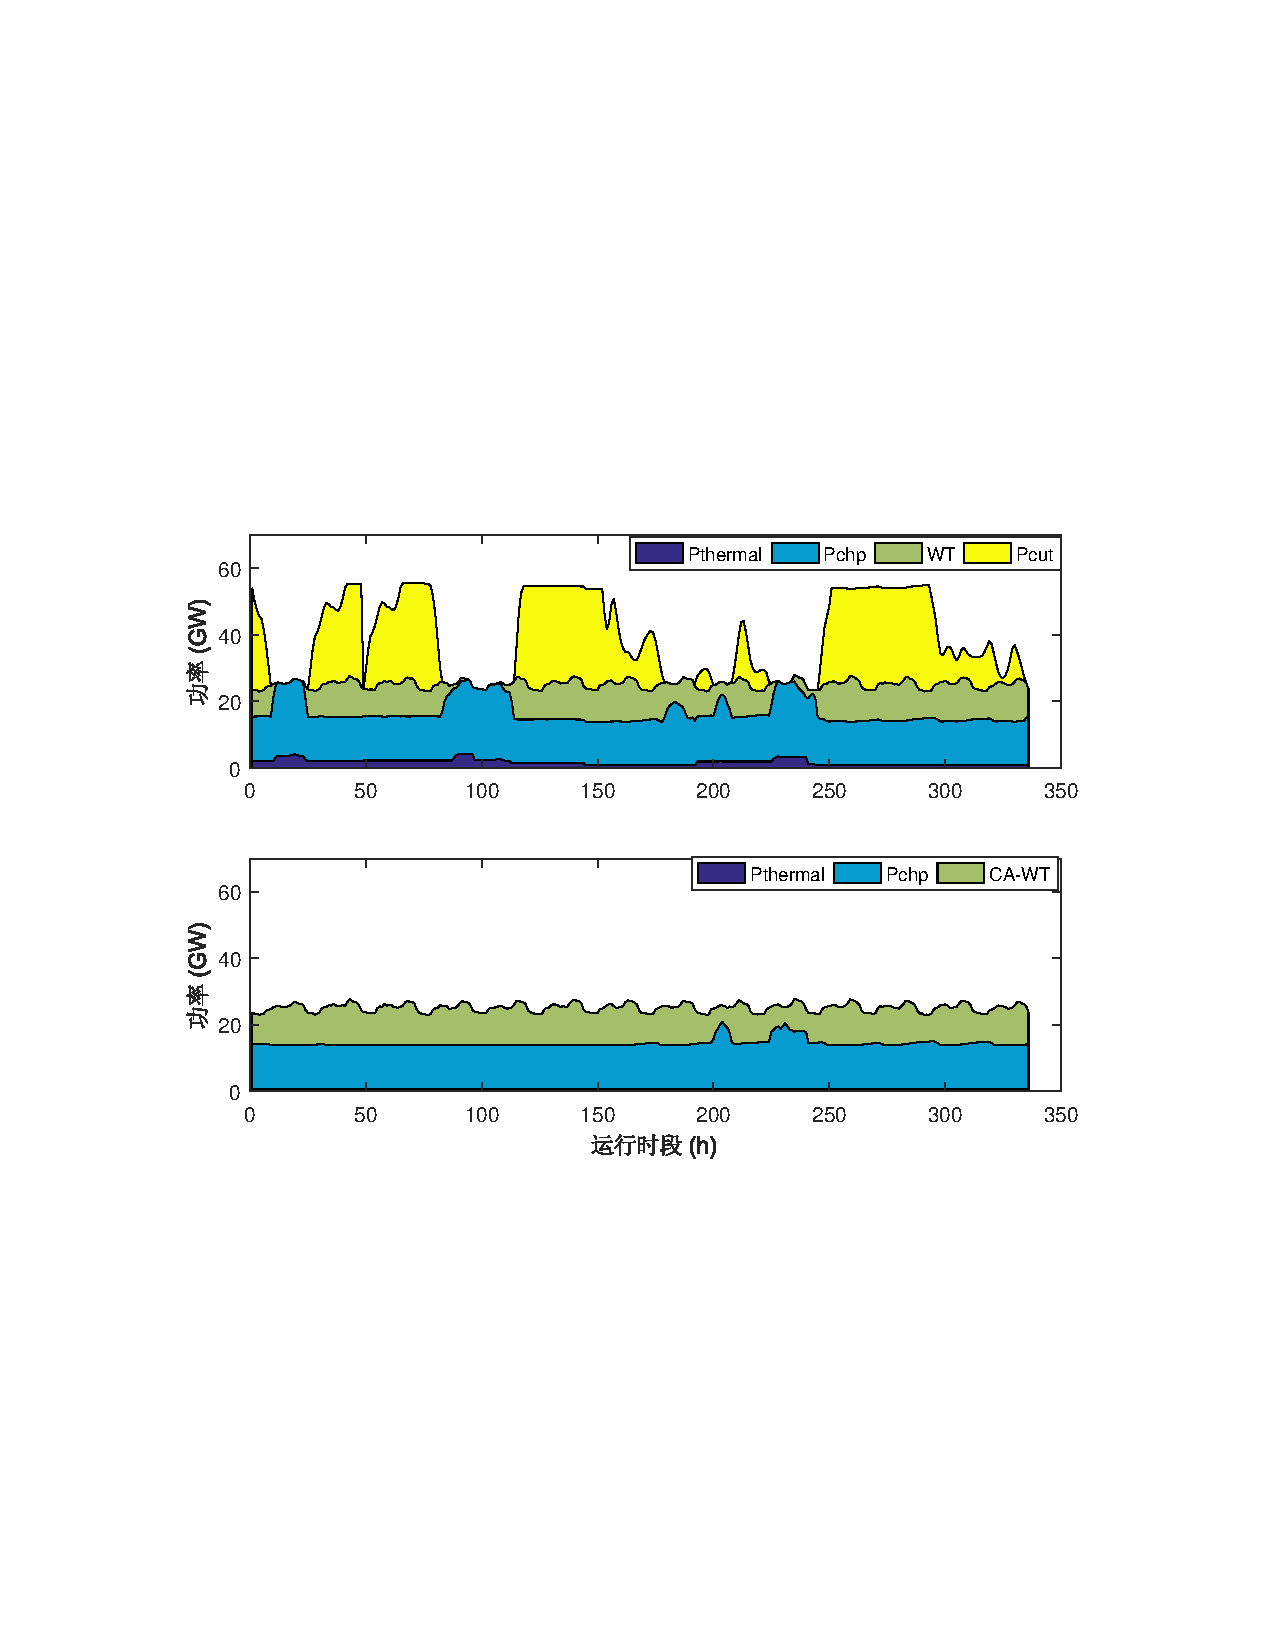
\includegraphics[scale=0.85]{figures/Chap5-Power-Balance-40G-WT.pdf}
  \caption{40GW传统风机与灵活风机电量平衡图}
  \label{fig:Power-Balance-40G-WT}
\end{figure}

\begin{figure}[H] % use float package if you want it here
  \centering
  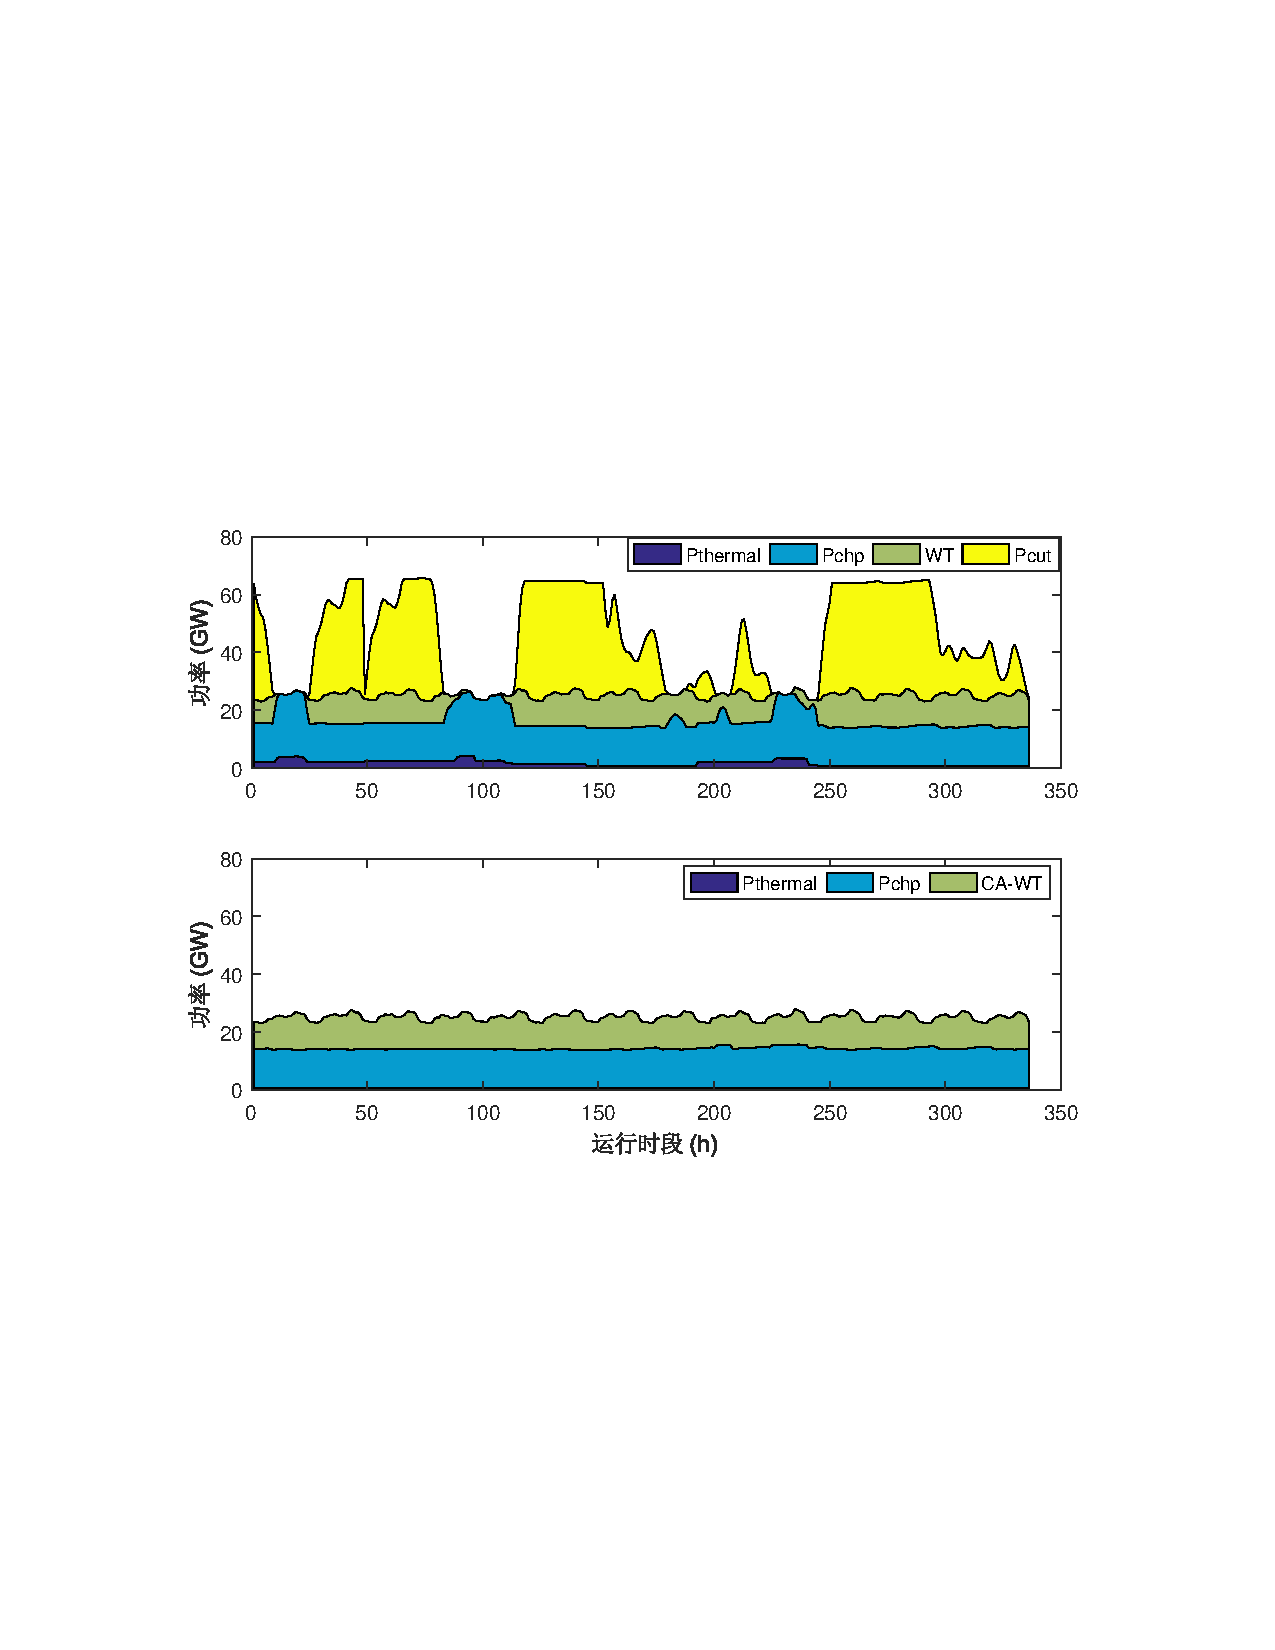
\includegraphics[scale=0.85]{figures/Chap5-Power-Balance-50G-WT.pdf}
  \caption{50GW传统风机与灵活风机电量平衡图}
  \label{fig:Power-Balance-50G-WT}
\end{figure}
